%% LaTeX Template for ISIT 2024
%%
%% by Stefan M. Moser, October 2017
%% (with some modifications by Tobias Koch, November 2023)
%% 
%% derived from bare_conf.tex, V1.4a, 2014/09/17, by Michael Shell
%% for use with IEEEtran.cls version 1.8b or later
%%
%% Support sites for IEEEtran.cls:
%%
%% http://www.michaelshell.org/tex/ieeetran/
%% http://moser-isi.ethz.ch/manuals.html#eqlatex
%% http://www.ctan.org/tex-archive/macros/latex/contrib/IEEEtran/
%%
\documentclass[twoside]{article}

\usepackage{aistats2025}

%% depending on your installation, you may wish to adjust the top margin:
%\addtolength{\topmargin}{9mm}

%% depending on your installation, you may wish to adjust the top margin:
%\addtolength{\topmargin}{9mm}

%%%%%%
%% Packages:
%% Some useful packages (and compatibility issues with the IEEE format)
%% are pointed out at the very end of this template source file (they are 
%% taken verbatim out of bare_conf.tex by Michael Shell).
%
% *** Do not adjust lengths that control margins, column widths, etc. ***
% *** Do not use packages that alter fonts (such as pslatex).         ***
%
\usepackage[utf8]{inputenc} 
\usepackage[T1]{fontenc}
\usepackage{url}
\usepackage{ifthen}
\usepackage{cite}
\usepackage[cmex10]{amsmath} % Use the [cmex10] option to ensure complicance
                             % with IEEE Xplore (see bare_conf.tex)

%% Please note that the amsthm package must not be loaded with
%% IEEEtran.cls because IEEEtran provides its own versions of
%% theorems. Also note that IEEEXplore does not accepts submissions
%% with hyperlinks, i.e., hyperref cannot be used.
\usepackage{amsthm,mathrsfs}
\usepackage{mathcomSTEv4}
\usepackage{makecell}
\usepackage{multirow}
\usepackage[T1]{fontenc}
\usepackage{cite}
\usepackage{enumerate}

\usepackage{enumitem}
\usepackage[utf8]{inputenc} 
\usepackage[T1]{fontenc}
\usepackage{url}              % provides \url{...}
%\usepackage{ifthen}          % provides \ifthenelse
\usepackage{cite}             % improves presentation of citations

\usepackage[cmex10]{amsmath}  % Use the [cmex10] option to ensure complicance
                              % with IEEEXplore (see bare_conf.tex)
%\interdisplaylinepenalty=1000 % As explained in bare_conf.tex
%\usepackage{mleftright}       % fix to wrong spacing of \left-,
%\mleftright                   % \middle- \right-commands 
\usepackage{pgfplots}
\pgfplotsset{compat=1.18}
\usepackage{pgfplotstable}
\usepackage{xcolor}
\usepackage{graphicx}         % provides \includegraphics{...} to
\usepackage{mathtools}
\DeclarePairedDelimiter{\ceil}{\lceil}{\rceil}
\DeclarePairedDelimiter\floor{\lfloor}{\rfloor}
%\usepackage[toc,page]{appendix}
%\usepackage{caption}
\usepackage{amsfonts}
\usepackage{bm}
\usepackage{bbm}
\usepackage{makecell}
\usepackage{multirow}
 \usepackage{amssymb}
\usepackage{txfonts}
\usepackage[T1]{fontenc}
\usepackage{tikz}
\usepackage[scr=dutchcal]{mathalfa}
\usepackage{ textcomp }
\usepackage{floatflt}
\usepackage{amsthm}                              % include graphics (pdf format)
\usepackage{booktabs}



\theoremstyle{definition}
\newtheorem{Theorem}{Theorem}
\newtheorem{Proposition}{Proposition}
\newtheorem{Lemma}{Lemma}
\newtheorem{Corollary}{Corollary}
\newtheorem{Example}{Example}
%
\newtheorem{Remark}{Remark}
%
\newcommand{\ste}{ \color{orange}}
\newcommand{\Tsf}{\mathsf{T}}

\newtheorem{Definition}{Definition}

\newtheorem{Proof}{Proof}
\newcommand{\indep}{\rotatebox[origin=c]{90}{$\models$}}
\newtheorem{Claim}{Claim}


%-------------------------------
\newcommand{\Esf}{\mathsf{E}}
\newcommand{\Qsf}{\mathsf{Q}}

%------------------------------- 
\interdisplaylinepenalty=2500 % As explained in bare_conf.tex


%%%%%%
% correct bad hyphenation here


% ------------------------------------------------------------
\begin{document}
\twocolumn[



% %%% Single author, or several authors with same affiliation:
% \author{%
%  \IEEEauthorblockN{Andrew R.~Barron}
%  \IEEEauthorblockA{Department of Statistics and Data Science\\
%                    Yale University\\
%                    New Haven, CT, USA\\
%                    Email: andrew.barron@yale.edu}
% }


%%% Several authors with up to three affiliations:

\aistatstitle{The Interactive Hypothesis Testing Problem}

\aistatsauthor{%
Mahshad Shariatnasab\textsuperscript{1}\thanks{Email: \texttt{mshar075@fiu.edu}} \And
Farhad Shirani\textsuperscript{1}\thanks{Email: \texttt{fshirani@fiu.edu}} \And
Stefano Rini\textsuperscript{2}\thanks{Email: \texttt{stefano.rini@nycu.edu.tw}}}

\aistatsaddress{%
\textsuperscript{1}Knight Foundation School of Computing and Information Sciences, Florida International University \\
\textsuperscript{2}Electrical and Computer Engineering Dept., National Yang-Ming Chiao Tung University}
]


%%% Many authors with many affiliations:
% \author{%
%   \IEEEauthorblockN{Andrew R.~Barron\IEEEauthorrefmark{1},
%                     Claude E.~Shannon\IEEEauthorrefmark{2},
%                     David Slepian\IEEEauthorrefmark{2},
%                     and Jacob Ziv\IEEEauthorrefmark{2}\IEEEauthorrefmark{3}}
%   \IEEEauthorblockA{\IEEEauthorrefmark{1}%
%                    Department of Statistics and Data Science, Yale University, New Haven, CT, USA,
%                     andrew.barron@yale.edu}
%   \IEEEauthorblockA{\IEEEauthorrefmark{2}%
%                     Bell Telephone Laboratories, Inc.,
%                     Murray Hill, NJ, USA,
%                     \{csh,dsl,jz\}@bell-labs.com}
%   \IEEEauthorblockA{\IEEEauthorrefmark{3}%
%                     Department of Electrical Engineering, Technion---Institute of Technology, Haifa, Israel,
%                     jz@ee.technion.ac.il}
% }

\begin{abstract}




 chatGPT chat link
\url{https://chat.openai.com/share/522ae6a3-e3cd-4c94-8722-441dd080bef3}

\end{abstract}

\section{Introduction}

{\ste SR2ALL: tone down privacy. Make the constrained more general. Let's call it a sampling constraint and say that it generalizes communication, complexity and privacy constraint, although it does not exhaust all notions of privacy and security. For complexity, can also mention implementation using decision trees which is common in networking for threat detection.}

%\textcolor{red}{(Will change)}
%Binary hypothesis testing is a statistical inference problem concerning the decision between two distinct probability distributions of the observed data. This paper focuses on distinguishing between two probability distributions when access to full data is limited. The main approach involves an agent sending queries to a device and analyzing the responses received. An application of this approach is in detecting bots, where the agent aims to determine whether the data source is a human or a bot based on limited information from these interactions. Beyond bot detection, we can find applications in other areas such as, source coding, differential privacy \cite{asoodeh2021three, puranik2022generalized}, machine learning \cite{berg2020binary}, and cryptographic protocols \cite{chakraborty2023novel}. 


\begin{figure*}
\begin{center}
\includegraphics[height=2.1in]{Overview.pdf}
\caption{\textcolor{red}{This will change}}
\label{fig:Overview}
\end{center} 
\end{figure*} 


%This paper focuses on distinguishing between two probability distributions when access to full data is limited. The main approach involves an agent sending queries to a device and analyzing the responses received. A key application of this approach is in detecting bots. In such scenarios, the agent aims to determine whether the data source is a human or a bot based on limited information from these interactions. This process is shown in Figure \ref{fig:Overview}. 

\vspace{2cm}

\noindent
{\bf Notation:}
 We represent random variables by capital letters such as $X, U$ and their realizations by small letters such as $x, u$. Sets are denoted by calligraphic letters such as $\mathcal{X}, \mathcal{U}$. The random variable $\mathbbm{1}_{\mathcal{E}}$ is the indicator function of the event $\mathcal{E}$.
 The set of numbers $\{n,n+1,\cdots, m\}, n,m\in \mathbb{N}$ is represented by $[n,m]$. Furthermore, for the interval $[1,m]$, we use the shorthand notation $[m]$ for brevity. 
 For a given $n\in \mathbb{N}$, the $n$-length vector $(x_1,x_2,\hdots, x_n)$ is written as $x^n$. 
% In the following, lowercase boldface letters (eg. $\zv$) are used for column vectors and uppercase boldface letters (e.g., $\Mv$) designate matrices. 
% %
% %Sets are indicated with calligraphic letters. 
% %
% The all-zero vector of dimension $d$ is indicated as $\zerov_d$.
% %
% We also adopt the shorthands $[m:n] \triangleq \{m, \ldots, n\}$
% and  $[n] \triangleq \{0, \ldots, n\}$. 
% %
% The $p$-norm of the vector $\xv$ is indicated as $\| \xv\|_p$.


\section{Problem Formulation}
This work considers the indirect hypothesis testing scenario shown in Figure \ref{fig:Overview}. The scenario models various applications of interest including bot detection \cite{acien2022becaptcha, akrout2019hacking}, privacy-preserving data analysis \cite{liao2017hypothesis,bloch2021overview}, distributed machine learning \cite{yin2021comprehensive}, and secure multi-party computation tasks \cite{lindell2020secure}. In the sequel, we describe the general problem formulation, and explain the underlying variables and operations in the context of bot detection as a motivating application. 

%  Alice observes a sequence of random variables generated according to one of the two (known) hypotheses, and Bob wishes to decide which hypothesis is true by querying Alice about her observed sequence.

The IHT scenario involves two agents, Alice and Bob. In the context of bot detection (e.g., CAPTCHA v3 \cite{google_recaptcha_v3}), Bob represents a website moderator and his objective is to decide whether a visitor to the website is a human user (null hypothesis) or an automated agent (alternative hypothesis). Alice represents the user's browser, which can observe a sequence of actions such as mouse movements, scrolls, and clipboard actions such as copy, cut, and paste. Alice cannot directly communicate her observations to Bob due to privacy constraints and potential bandwidth limitations. Consequently, Bob can make queries regarding Alice's observations to decide between the two hypotheses. Ideally, Bob wishes to achieve three objectives: i) decide on the correct hypothesis in a minimal amount of time. For instance, in bot detection, classification must be completed in hundreds of milliseconds, and the rate at which Alice observes symbols $Z_i$ is several milliseconds;
ii) achieve maximal detection accuracy. For instance, in bot detection, false negatives in detecting automated agents may lead to significant financial damage \cite{isemag}, and false positives may degrade user experience; and iii) collect the minimal information necessary to achieve the previous two objectives  to ensure compliance with privacy related regulations and restrictions such as European Union's GDPR and California's privacy act \cite{park2019changing}. 

Formally, Alice observes a sequence of random variables $Z^n$. To keep the results tractable, we assume that $Z^n$ is an independent and identically distributed (IID) sequence. Under the null hypothesis ${H}_0$, the sequence is generated according to a distribution $P_X$, and under the alternative hypothesis $H_1$, the sequence is generated according to $P_Y$, where $P_X$ and $P_Y$ are defined on the same finite alphabet $\mathcal{Z}$. Bob wishes to decide between the null and alternative hypotheses by sequentially querying Alice. Each query is in the form of a subsequence $z^m$, and Alice responds by sending back the time index of the first time that she observes the queried subsequence after receiving Bob's query. For instance, in bot detection, Bob may ask a query of the form `R,L,U', where `R', `L' and `U' represent right, left, and up mouse movements, respectively. Assume that after receiving Bob's query, Alice's observed sequence of  mouse movements is $Z_1=R,Z_2=R,Z_3=L,Z_4=R,Z_5=R,Z_6=L,Z_7=U,Z_8=R,Z_9=L$. Then, she sends back the query response $T=7$ since $Z_5,Z_6,Z_7=RLU$ is the first instance that the queried sequence is observed.  


\begin{Definition}[\textbf{Query Function and Query Response}]
\label{def:time}
Let $\Delta\in \mathbb{N}$, and define the set of admissible $\Delta$-length queries as $\mathcal{Q}_{\Delta}\triangleq \{z^{\Delta}| z_i \in \mathcal{Z}\}$. Given a 
 random process $Z_1, Z_2, \ldots$ and a query sequence $z^{\Delta}\in \mathcal{Q}_{\Delta}$,  the query response at time $t\in \mathcal{N}$ is defined as: 
\begin{align*}
    &T_j(z^{\Delta},t) = \argmin_{j: t+\Delta\leq  j} \{j| Z_{j-\Delta+1}^{j}=z^{\Delta}\}. 
\end{align*}
%Here, $T_j$ serves as a shorthand for $T_j(Z,\sigma_j)$, with each $T_j$ corresponding to a distinct pattern or subsequent definition of length $\Delta$.
\end{Definition}

The $i$th query, sent by Bob to Alice at time $t_i$, is parametrized by a finite sequence $z^{m_i}\in \mathcal{Z}^*, 
m_i, i\in \mathbb{N}$, where $\mathcal{Z}^*\triangleq \{z^m| z_i\in \mathcal{Z}, i\in [m], m\in \mathbb{N}\}$ is the set of all finite-length sequences on the set $\mathcal{Z}$. After receiving the query $z^{m_i}$, Alice sends back the time index $T_i$ of the first instance where $z^{m_i}$ is observed in the sequence $Z_{{t_i}}, Z_{t_{i+1}},\cdots$. Bob then decides to either declare one of the two hypotheses as the true hypothesis based on the received query responses $T_1,T_2,\cdots,T_i$, or to continue asking additional queries. 

Formally, ...



\textcolor{red}{explain a high-level overview of the problem, in the context of bot detection, mention Figure and high-level overview of the problem. If high-level overview is given here, then the rest of the application-related descriptions in future paragraphs can be very brief, otherwise, we can distribute the descriptions to each definition itself.}

In the IHP problem formulation the source coding is not available to the agent and the agent only can send queries $Q_i$ to the source based on the query responses $T_i$ he can decide whether the source is based on distribution $H_0$ or $H_1$. To facilitate explanation, and provide justifications for the model assumptions, we describe the model by focusing on the scenario of bot detection. 


In a typical bot detection scenario, consider Bob as a website administrator and Alice representing a device interacting with the website. Bob's objective is to ascertain whether Alice is a human user or an automated agent. To achieve this, Bob employs a web socket that monitors specific user actions, such as mouse movements (scroll events, and clipboard interactions like cut, paste, and copy and etc.).

However, due to privacy concerns, Bob's script is designed to respect Alice's privacy. It does not transmit all the collected information back to the server. Instead, Bob's system is structured to respond to specific queries about the data it collects. This selective approach allows Bob to gather relevant information without compromising the privacy of Alice.

Bob utilizes the responses to these targeted queries to conduct a binary hypothesis test. This test is designed to determine the nature of Alice's interaction with the website - whether it is human-driven or bot-driven. This setup epitomizes an IHT problem, where the full dataset is not directly accessible, but insights are drawn from specific, limited data points. This process is shown in Figure \ref{fig:Overview}. 






%\textcolor{red}{explain a high-level overview of the problem, in the context of bot detection, mention Figure and high-level overview of the problem. If high-level overview is given here, then the rest of the application-related descriptions in future paragraphs can be very brief, otherwise, we can distribute the descriptions to each definition itself.}

\vspace{1cm}
{\ste: changed this part to be more compact and general. Once we agree, we redo the figure.}

\vspace{1cm}

% \begin{Definition}[\textbf{Null and alternative hypothesis}]

% Consider two hypotheses \( H_0 \) and \( H_1 \) which correspond to the two possible underlying distributions, \( P_X \) and \( P_Y \), governing the samples. In other words, we have:
% \begin{align*}
% H_0: Z \sim P_X(\cdot), \\
% H_1: Z \sim P_Y(\cdot),
% \end{align*}
% where \( Z \) takes values in a finite set \( \mathcal{Z} \). We also assume that the distributions $P_X$ and $P_Y$ are known to both the agents.

% \end{Definition}


%\begin{Definition}[\textbf{Null and Alternative Hypothesis}]
%At each time \( n = 1, 2, \ldots \) let $Z_n \in \mathcal{Z}$ be a outcomes that are characterized by the hypothesis $H_0$.
%\begin{align*}
%    Z \sim P_1(\cdot)
%\end{align*}
    
%\end{Definition}




%\textcolor{red}{(if the high level overview is not given in the beginning, then we need more detailed description of the bot detection problem here. e.g., For instance: consider a setup where Bob is a website administrator, and Alice represents a device visiting the website. Bob wishes to determine whether Alice is controlled by a human user or an automated agent. To this end, Bob uses a web socket which collects specific user actions, such as mouses movements, scrolls, clipboard actions (cut, paste, copy, etc.). To preserve Alice's privacy and abide by regional privacy laws, Bob's script does not send back all the information that it collects, rather, it responds to specific queries that Bob sends regarding the collected data. Bob uses the query responses to perform a  binary hypothesis test and determine the nature of Alice's visit. A formal statement of this \textit{indirect hypothesis testing} problem is provided below. }



%These responses, as the sequence $T$, are received by Bob one at a time. Bob's goal is to decide between the two possible distributions, $P_X$ and $P_Y$, where $P_X$ and $P_Y$ are the probability distribution of bot and human queries.
%In the subsequent definition, we will elaborate on how Alice encodes the vector $Z$ into the vector $T$.


% \begin{Definition}[\textbf{Query Responses}]

% Consider a sequence $Z=\{Z_1, Z_2, \ldots, Z_n\}, n \in \mathbb{N}$. For a series of different combinations or permutations $\{\sigma_1, \sigma_2, \ldots, \sigma_m\}, m \in \mathbb{N}$ derived from a finite set ${\Sigma}$, we define a corresponding series of functions $\{T_j\}_{j=1}^m, j\in[m]$. Each function $T_j$ is associated with a specific permutation $\sigma_j$ and is defined as follows:


% \begin{align*}
%     &T_j(X;\sigma_j) = \argmin_{i} \{ i \mid 1 \leq i \leq n-|\sigma_j|+1, 
%     \\& (Z_i, Z_{i+1}, \ldots, Z_{i+|\sigma_j|-1})= \sigma_j \}
% \end{align*}    

% In this problem formulation without loss of generality, we use $T_j$ instead of $T_j(X,\sigma_j)$.
% \end{Definition}






%The probability of observing \( y \) after performing an experiment \( x \) under hypothesis \( h \) is denoted by \( p_{x}^{h}(y) \), that is,

%\[
%p_{x}^{h}(y) \triangleq P(Y_n = y | H = h, X_n = x).
%\]

In this problem formulation, Alice generates a random process $Z_1,Z_2,\cdots$. At any given time $n\in \mathcal{N}$, Bob may ask Alice a query parameterized by a sequence $(z_1,z_2,\cdots,z_k)$, where $k\in \mathbb{N}$ and $z_i\in \mathcal{Z}$. Having received the query, Alice sends back a variable $T$ which is equal to the number of sequence symbols $Z_n,Z_{n+1},\cdots,Z_{m}$ observed until the query sequence is observed for the first time. 

\begin{Remark}
    Consider a scenario where Alice generates a binary sequence \( z_1, z_2, z_3, z_4, z_5 = 0, 1, 1, 1, 0 \) from the set \( \mathcal{Z} = \{0, 1\} \). Bob, intending to identify a specific pattern in Alice's sequence, sends a series of queries. Suppose Bob's queries are \( q_1, q_2, q_3=  0, 1, 0 \) (a specific pattern he is looking for in the sequence). 

Alice's responses to these queries, denoted by \( T \), are determined by the earliest occurrence of each query pattern. For the query pattern \( 0 \), the earliest occurrence in Alice's sequence is at position 1 (for \( Z_1 \)). For the pattern \( 1 \), it is at position 2 (for \( Z_2 \)), and for the pattern \( 0 \) again, it occurs at position 5 (for \( Z_5 \)). Therefore, Alice's response to these queries will be \( T = 1, 2, 5 \).
\end{Remark}



Let us assume that at a given time $t \in \mathbb{N}$, Bob receives a query response $T_{k_t}$, where $k_t$ is the total number of query responses received up to time $t$. Bob has two choices, one is to declare the output of the Hypothesis test by determining either the null or alternative hypothesis as the ground truth, or to continue sending new queries by choosing a new query sequence. We model Bob's operation by two functions, namely, the query function and the identification function. The pair of functions is called an identification strategy. These are formally defined in the following. 

%When Bob receives query responses $ \{T_1, T_2, T_3, \ldots\} $, it utilizes query functions $x_t(\cdot)$ and identification function $ \text{Id}_t(\cdot)$, for $t \in \mathbb{N}$. The query function $ x_t(T^{t-1})$ takes as input the encoder output $T^{t-1}$ up to time $t-1$ and outputs the next experiment $ \sigma_t$. Upon receiving the response $T^t$, the identification function $ \text{Id}_t(T^t)$ compares the probability of $T^t$ with Alice probability distribution $P_X$ and Bob probaility distribution $P_Y$. It then either decides between hypotheses $ H_0$ and $H_1$, or indicates that the identity cannot be determined yet, suggesting that the agent should conduct the next experiment. The Identification function can take values in $\hat{H} \cup \{e\}$, where $\hat{H} \in \{H_0, H_1\}$.


\begin{Definition}[\textbf{Identification Strategy}]
 Let $\Delta\in \mathbb{N}$. An identification strategy consists of a pair of sequences of query functions and identification functions   $x_i : \mathbb{N}^{i-1} \to \mathcal{Q}_{\Delta}$ and $Id_i:\mathbb{N}^{i}\to \{0,1,c\}, i\in \mathbb{N}$, respectively. The sequence of pairs $(x_i,Id_i)_{i\in \mathbb{N}}$ is called an identification strategy. 

 The output of the (fixed) function $x_1()$ represents Bob's query sequence at time $t=1$, and the output of $x_{i}(T^{i-1})$ represents Bobs query sequence at time $t=T_{i-1}$, where $T_i$ is defined in Definition \ref{def:time}. We define $K_t\triangleq i-1$.  Having received query responses $T_1,T_2,\cdots,T_i$, if $Id_{i}(T^i)\in \{0,1\}$, then Bob outputs the hypothesis $H_{Id_{i}(T^i)}$ as his estimate of the ground-truth, otherwise, if $Id_{i}(T^i)=c$, Bob sends query $x_{i+1}(T^{i})$.  


 
% identification function is a function of the form $Id_i:  \mapsto \hat{H} \cup \{e\}$, where $x_t(T^{t-1})$ outputs the next experiment $\sigma_t$ at the time $t$ and identification $Id_t(T^t)$ either outputs the $H_0$ and $H_1$ or outputs `e' in which case the information is not enough and further sequence is needed. 
%Let $t\in \mathbb{N}$, and define $K_t$ as the random variable corresponding to the number of queries 
\end{Definition}

\begin{Remark}
In the context of the identification strategy, the nature of the queries sent by Bob can be either adaptive or non-adaptive. A non-adaptive query strategy implies that the sequence of queries is predetermined and fixed before the test begins, regardless of the responses received. For example, if Bob decides to send the queries \(0, 1, 0\) in sequence irrespective of Alice's responses, this represents a non-adaptive approach.

On the other hand, an adaptive query strategy allows Bob to adjust his queries based on the responses received from Alice. For instance, if Bob's initial query is \(0\) and, based on Alice's response, he decides to follow up with a \(1\) or another \(0\), this approach is adaptive as it adapts to the information gathered during the testing process.

In this paper, both scenarios are considered. The non-adaptive approach is useful for situations where a predefined sequence of queries is necessary, while the adaptive approach allows for more flexibility and potentially more efficient identification strategies based on the evolving nature of the responses.
\end{Remark}

\begin{Definition}[\textbf{Type-I Error Probability}]
The Type-I error probability, denoted as \( P_{1|0}(Id_{T_i}, i) \), is defined as the probability that the identification function \( Id_{T_i} \) decides in favor of \( H_1 \) when the true hypothesis is \( H_0 \) based on the observations up to time \( i \). Formally:
$$
P_{1|0}(Id_{T_i}) = P_X(Id_{T_i} = 1).
$$
\end{Definition}

\begin{Definition}[\textbf{Type-II Error Probability}]
The Type-II error probability, denoted as \( P_{0|1}(Id_{T_i}, i) \), is defined as the probability that the identification function \( Id_{T_i} \) decides in favor of \( H_0 \) when the true hypothesis is \( H_1 \) based on the observations up to time \( i \). Formally:
$$
P_{0|1}(Id_{T_i}) = P_Y(Id_{T_i} = 0).
$$
\end{Definition}


\begin{Definition}[\textbf{Objective Function}]

Let \( T_i \) be the response at the \( i \)-th time step in the identification strategy comprising sequences of query functions \( x_i : \mathbb{N}^{i-1} \to \mathcal{Q}_{\Delta} \) and identification functions \( Id_i : \mathbb{N}^i \to \{0, 1, c\} \). Define the objective function to minimize the probability of incorrect identification as:
$$
\min \quad \mathcal{E}=  P_{0|1}(Id_{T_i}) + P_{1|0}(Id_{T_i}),
$$
where \( P_{1|0}(Id_{T_i}, i) \), is the probability that the identification function \( Id_{T_i} \) decides in favor of \( H_1 \) when the true hypothesis is \( H_0 \), and \( P_{0|1}(Id_{T_i}, i) \), is the probability that the identification function \( Id_{T_i} \) decides in favor of \( H_0 \) when the true hypothesis is \( H_1 \) based on the observations up to time \( i \)
\end{Definition}


This objective function aims to find an optimal balance between minimizing the probability of falsely rejecting the null hypothesis (Type-I error) and minimizing the probability of falsely accepting it (Type-II error) within the constraints of the given identification strategy.

\vspace{1cm}
{\ste: changed from here}

\vspace{1cm}
Consider the binary hypothesis testing in which a remote observer -- Alice  -- has access to a set of observations from the process $\{Z_t \}_{t \in [T]}=Z^T$ comprised of i.i.d. entries from two possible hypothesis:
\begin{align*}
\Hcal_0: & \ \ Z \sim P(\cdot) \\
\Hcal_1: & \ \ Z \sim Q(\cdot),
\end{align*}
over the same finite alphabet $\Zcal$ with cardinality $\|\Zcal\|\subseteq \Nbb$.
%
A central detector -- Bob -- is tasked with detecting which hypothesis is correct through a set of \emph{query-hit exchanges}  with Alice.
%
A \emph{query} $Q=z^l$ is a sequence of length $l \in \Nbb$ of the element of $\Zcal$. 
%
Given the source sequence $Z^T$, the query hit-time $\Tsf(Q,Z^T)$ is  define as 
%
\ea{
\tsf(Q|Z^T) =  \argmin_{j: \ \  t+l \leq  j}  \ \ \lcb j \ | \ Z_{j-l+1}^{j}=z^{l}\rcb. 
\label{eq:query zero}
}
for $Q=z^l$.
%
%
A \emph{set} of $K$ successive query-hit exchanges, queries being produced by Bob and hits by Alice, is defined
%more compactly  denoted as
\ea{
\lcb (Q_k,\tsf_k)  \ | \  Z^T \rcb_{k \in [K]}. 
\label{eq:set of qh}
}
where $\tsf_1$ is obtained as is 
\ea{
\tsf_k = \tsf(Q_k|Z^T_{\tsf_{k-1}})
}


\begin{Remark}
    {\ste say query do not superpose}
\end{Remark}
Given the set of $K$ query-hits exchanges as in \eqref{eq:set of qh}, the detector choses an hypthosis 
\ea{
\hh = \hh \ \lb \lcb (Q_k,\tsf_k)  \ | \  Z^T \rcb_{k \in [K]}.  \rb  \in \{0,1\}.
}
For compactess, let us define a \emph{querying strategy} of length $K$ as the tuple  
\ea{
\Qsf_K = \lsb \{Q_k\}_{k\in [K]}, \hh \rsb.
}
\subsection{Performance analysis}
%
%{\ste I prefer the chernoff information approach here}
%\vspace{1cm}
Given a querying strategy $\Qsf$ let us define -- as costumary-- the type I and type II errors as 
\ea{
\al_k & = P[\hh \neq \Hcal | \Hcal = 0] \\
\be_k & = P[\hh \neq \Hcal | \Hcal = 1].
}
Bob's objective is to choose the correct hypothesis with the highest probability and the shortest time. 
To harmonize these two objectives, we take an error exponent approach, that is we consider the exponent
\ea{
\Esf(\Qsf_K) = - \f 1 {\Ebb \lsb \sum_{k \in [K]}] \tsf_{k}\rsb}  \log \be_K,
}
and the Chernoff–Stein lemma-type maximization
\ea{
\Esf^*(\ep)  = \max_{\Qsf_K,  \ST \al_K\leq \ep}  \Esf(\Qsf_K),
}
that is we wish to maximize the error exponent of the type II errors, subject to the type I error to be at most $\ep$.
The maximization 

\subsection{Adaptive vs non-adaptive}

{\ste complete: we want both}

% 1111111111111111111111
% Q: 11
% H:? 1 2 3 4 5 X
% H:0 2 4 6

%\subsection*{Adaptive and Non-Adaptive \( Q \) Function}
{\ste
The function \( Q \) can be implemented in two distinct modes: Adaptive and Non-Adaptive. These modes dictate how the function \( Q \) operates based on its output and the subsequent actions of the agent. 

\begin{Definition}[\textbf{Non-Adaptive \( Q \)}]
In the Non-Adaptive implementation of \( Q \), the function is fixed and predefined before its execution. Once set, the agent does not modify or adjust the function based on the output it generates. This means that the function \( Q \) operates consistently throughout its application, without any alteration in response to the data it processes or the results it produces. 
\end{Definition}

\begin{Definition}[\textbf{Adaptive \( Q \)}]
Conversely, in the Adaptive implementation, the agent has the capability to adjust or modify the function \( Q \) based on its output. This means that the function \( Q \) is dynamic and can evolve in response to the data it encounters. This adaptability allows for a more flexible approach, potentially enhancing the efficacy of the function in various scenarios. However, in the context of binary sequences, the distinction between adaptive and non-adaptive \( Q \) is minimal. This is because, with binary sequences, the agent can reconstruct the entire sequence, making the adaptability of the function less impactful.
\end{Definition}

These definitions articulate the key differences between the two modes of operation for the function \( Q \) and provide insights into their respective utilities and limitations, particularly in the context of binary sequence analysis.
}


% \vspace{3cm}
% To measure the detection performance, we take Chernoff's approach. 
% %
% \vspace{1cm}
% {\ste must define the choice of query functions here: adaptive or not? how  do we handle it?}
% \vspace{1cm}
% %
% Assume that hypothesis $\Hcal = i$ is selected with probability $\pi_i$, than the \emph{error probability} is defined as
% \ea{
% P_e = \pi_0 P[\hh \neq \Hcal | \Hcal = 0] +  \pi_i P[\hh \neq \Hcal | \Hcal = i].
% }
% The error exponent is defined as 
% \ea{

% }

% \vspace{2cm}
% {\ste this formulation is more compact imo, since the decision is only at the end of things}
% \vspace{2cm}

% is a statistical inference problem
% concerning the decision between two distinct probability distributions of the observed data. Consider two hypotheses \( H_0 \) and \( H_1 \) which correspond to the two possible underlying distributions, \( P_X \) and \( P_Y \), governing the samples. In other words, we have:
% \begin{align*}
% H_0: Z \sim P_X(\cdot), \\
% H_1: Z \sim P_Y(\cdot),
% \end{align*}
% where \( Z \) takes values in a finite set \( \mathcal{Z} \). We also assume that the distributions $P_X$ and $P_Y$ are known to both the agents.



% %\begin{Definition}[\textbf{Null and Alternative Hypothesis}]
% %At each time \( n = 1, 2, \ldots \) let $Z_n \in \mathcal{Z}$ be a outcomes that are characterized by the hypothesis $H_0$.
% %\begin{align*}
% %    Z \sim P_1(\cdot)
% %\end{align*}
    
% %\end{Definition}


\subsection{A motivating scenario}

{\ste make this a recurring example. just it up here as a motivation but keep the setting open}
\vspace{1cm}

In a typical bot detection scenario, consider Bob as a website administrator and Alice representing a device interacting with the website. Bob's objective is to ascertain whether Alice is a human user or an automated agent, a decision critical for maintaining the integrity and security of the website. To achieve this, Bob employs a web socket that monitors specific user actions, such as mouse movements (scroll events, and clipboard interactions like cut, paste, and copy and etc.).

However, due to privacy concerns, Bob's script is designed to respect Alice's privacy. It does not transmit all the collected information back to the server. Instead, Bob's system is structured to respond to specific queries about the data it collects. This selective approach allows Bob to gather relevant information without compromising the privacy of Alice's visit.

Bob utilizes the responses to these targeted queries to conduct a binary hypothesis test. This test is designed to determine the nature of Alice's interaction with the website - whether it is human-driven or bot-driven. This setup epitomizes an \textit{indirect hypothesis testing} problem, where the full dataset is not directly accessible, but insights are drawn from specific, limited data points.

In this problem formulation, Alice generates a random process $Z_1,Z_2,\cdots$. At any given time $n\in \mathcal{N}$, Bob may ask Alice a query parameterized by a sequence $(z_1,z_2,\cdots,z_k)$, where $k\in \mathbb{N}$ and $z_i\in \mathcal{Z}$. Having received the query, Alice sends back a variable $T$ which is equal to the number of sequence symbols $Z_n,Z_{n+1},\cdots,Z_{m}$ observed until the query sequence is observed for the first time. This is formalized below:

\textcolor{red}{(if the high level overview is not given in the beginning, then we need more detailed description of the bot detection problem here. e.g., For instance: consider a setup where Bob is a website administrator, and Alice represents a device visiting the website. Bob wishes to determine whether Alice is controlled by a human user or an automated agent. To this end, Bob uses a web socket which collects specific user actions, such as mouses movements, scrolls, clipboard actions (cut, paste, copy, etc.). To preserve Alice's privacy and abide by regional privacy laws, Bob's script does not send back all the information that it collects, rather, it responds to specific queries that Bob sends regarding the collected data. Bob uses the query responses to perform a  binary hypothesis test and determine the nature of Alice's visit. A formal statement of this \textit{indirect hypothesis testing} problem is provided below. }



%These responses, as the sequence $T$, are received by Bob one at a time. Bob's goal is to decide between the two possible distributions, $P_X$ and $P_Y$, where $P_X$ and $P_Y$ are the probability distribution of bot and human queries.
%In the subsequent definition, we will elaborate on how Alice encodes the vector $Z$ into the vector $T$.



\section{Preliminaries}
{\ste update notation when we all agree}

\vspace{1cm}

\begin{Lemma}[Neyman-Pearson Lemma]
\label{eq:Neyman-Pearson Lemma}
Let \( T_1, T_2, \ldots, T_k \) be the observed responses from a sequence of queries based on the data \( Z_1, Z_2, \ldots, Z_n \), where \( Z_i \) are i.i.d. according to a probability distribution \( Q \). Consider the decision problem corresponding to the hypotheses \( Q = P_X \) (for the underlying data \( Z \)) versus an alternative distribution \( P_Y \) (representing a different hypothesis for \( Z \)). Define a decision region \( A_k(\lambda) \) for the observed query responses as:
$$
A_k(\lambda) = \left\{ t^k : \frac{\mathbb{P}(T_1, T_2, \ldots, T_k | Q = P_X)}{\mathbb{P}(T_1, T_2, \ldots, T_k | Q = P_Y)} > \lambda \right\}.
$$
Let \( \alpha^* = \mathbb{P}^k(A_k(\lambda)^c | Q = P_X) \) and \( \beta^* = \mathbb{P}^k(A_k(\lambda) | Q = P_Y) \) be the probabilities of Type-I and Type-II errors, respectively, for decision region \( A_k(\lambda) \). For any other decision region \( B_k \) with associated probabilities of error \( \alpha \) and \( \beta \), if \( \alpha \leq \alpha^* \), then \( \beta \geq \beta^* \).
\end{Lemma}


\begin{proof}
Consider decision regions \( A_k(\lambda) \) as defined in the lemma for the observed query responses, and any other acceptance region \( B_k \subseteq \mathcal{T}^k \), where \( \mathcal{T}^k \) is the space of all possible sequences of \( k \) query responses. Let \( \phi_{A_k} \) and \( \phi_{B_k} \) be the indicator functions of \( A_k \) and \( B_k \), respectively. 

For all sequences of query responses \( t^k = (t_1, t_2, \ldots, t_k) \), the likelihood ratio test asserts that:
\begin{align*}
(\phi_{A_k}(t^k) - \phi_{B_k}(t^k))\left(\mathbb{P}(t^k | Q = P_X) - \lambda \mathbb{P}(t^k | Q = P_Y)\right) \geq 0.
\end{align*}
This inequality holds true because \( \phi_{A_k}(t^k) \) is 1 when \( t^k \) favors \( Q = P_X \) more strongly than \( Q = P_Y \) by a factor of more than \( \lambda \), and 0 otherwise. The same logic applies to \( \phi_{B_k}(t^k) \).

Summing over the entire space of query responses \( \mathcal{T}^k \), we obtain:
\begin{align*}
0 \leq \sum_{\mathcal{T}^k} (\phi_{A_k} \mathbb{P}_{P_X} - \lambda \phi_{A_k} \mathbb{P}_{P_Y} - \phi_{B_k} \mathbb{P}_{P_X} + \lambda \phi_{B_k} \mathbb{P}_{P_Y}).
\end{align*}

Rearranging the terms and translating them into Type-I and Type-II error probabilities for regions \( A_k(\lambda) \) and \( B_k \), we get:
\begin{align*}
\lambda (\beta - \beta^*) - (\alpha^* - \alpha) \geq 0,
\end{align*}
where \( \alpha^* \) and \( \beta^* \) are the Type-I and Type-II error probabilities for region \( A_k(\lambda) \), and \( \alpha \) and \( \beta \) are those for region \( B_k \).

Since \( \lambda \geq 0 \), it follows that if \( \alpha \leq \alpha^* \), then \( \beta \geq \beta^* \). This proves that the likelihood ratio test for the observed query responses is the most powerful test for distinguishing between \( Q = P_X \) and \( Q = P_Y \) under the constraint of a fixed Type-I error rate.
\end{proof}

\begin{Lemma}[Stein's Lemma \cite{}]
In the context of binary hypothesis testing for two probability distributions \( P_X \) and \( P_Y \) corresponding to hypotheses \( H_0 \) and \( H_1 \) respectively, Stein's Lemma relates the exponential decay rate of the Type-II error \( \beta \) to the Kullback-Leibler divergence \( D(P_X||P_Y) \). For a fixed Type-I error \( \alpha \) and \( n \) i.i.d. observations, Stein's Lemma states that:
$$
\lim_{n \rightarrow \infty} -\frac{1}{n} \log \beta_n = D(P_X||P_Y),
$$
where \( \beta_n \) is the Type-II error probability for \( n \) observations.
\end{Lemma}


\section{A Motivating example}

{\ste Rewrote this part: make it as communicative as possible.}

 \vspace{1cm}

% \textbf{Binary Example for Function \( Q \):}

Consider the binary setting in which 
\ea{
\Hcal_0 & \sim \Bcal(p_0) \\
\Hcal_1 & \sim \Bcal(p_1),
}
for some $p_0<p_1\leq 1/2 \in \Rbb^+$ without loss of generality, and let us consider the possible querying strategies.
%

\medskip
\noindent
{\bf Single query strategy}
One first approach that one imagines is that in which Bob produces a single query that is sufficient for reliable detection. 
%
Let us assume that the sequence is the all-zero sequence of length $l$ for some $l$ to be determined. 
%


\vspace{1cm}
{\ste complete}
\vspace{1cm}



\medskip
\noindent
{\bf Sequence reconstructive strategy.}

\vspace{1cm}
{\ste complete}
\vspace{1cm}




\medskip
\noindent
{\bf Non-adaptive querying strategy.}
Given a given query length $l$ and Lem. \ref{eq:Neyman-Pearson Lemma}, one first strategy would be to select the most discriminating query across the two hypotheses and repeat the query $K$ times.
%
Formally, 
\ea{
\max_{z^l}  \| \log (P(z^l))-\log (Q(z^l)) \| 
}
which -given the symmetry of the problem - corresponds to either the whole-zero and the whole-one query.  
%
Let us assume that we choose the query to be the whole-one query. 
%
Under this strategy, we have that the RV $\tsf_{k+1}=\Tsf_{k+1}-\Tsf_{k}$ in a success run of with probability of success $p_0^l$/$p_1^l$ under hypothesis $\Hcal_0$/$\Hcal_1$.
%

{\vspace{1cm}}
{\ste complete, what's the decay of the error probability with $l$}
{\vspace{1cm}}


\noindent
{\bf Long-queries first adaptive strategy.}



\noindent
{\bf Short-queries first adaptive strategy.}




\noindent
{\bf Optimal Adaptive querying strategy.*}
%
As an alternative strategy, consider the setting in which the query length 



Taking 
\vspace{3cm}

Consider a mouse trajectory represented in a binary format, for instance, \( \mathbf{T} = 010010110 \). In this sequence, each digit represents a state at a time instance, with '0' and '1' indicating different states or conditions.

Suppose the function \( Q \) is designed to notify whenever a '1' is encountered in the trajectory. For the given sequence \( \mathbf{T} \), applying \( Q \) would yield:

\[
Q(T_1, T_2, T_3, T_4, T_5, T_6, T_7, T_8, T_9) = \{2, 5, 6, 7, 9\}
\]

Here, the function \( Q \) selectively shares the indices of the trajectory where '1' appears. The output \( \{2, 5, 6, 7, 9\} \) indicates that '1' is found at the 2nd, 5th, 6th, 7th, and 9th positions in the original mouse trajectory sequence \( \mathbf{T} \). This example illustrates how \( Q \) can be used to extract and share specific, privacy-preserving information from the trajectory data.

\section{Main Results}
The primary objective of this paper is to develop a mathematical framework that enables the distinction between humans and bots, while concurrently preserving user privacy.

\subsection{Non-adaptive}
In the following figure we can see the average time to detect the hypothesis. In this setting the hypothesis I probability all the time is $0.5$ and we change the probability of hypothesis II.
\begin{figure}[htbp]
    \centering
    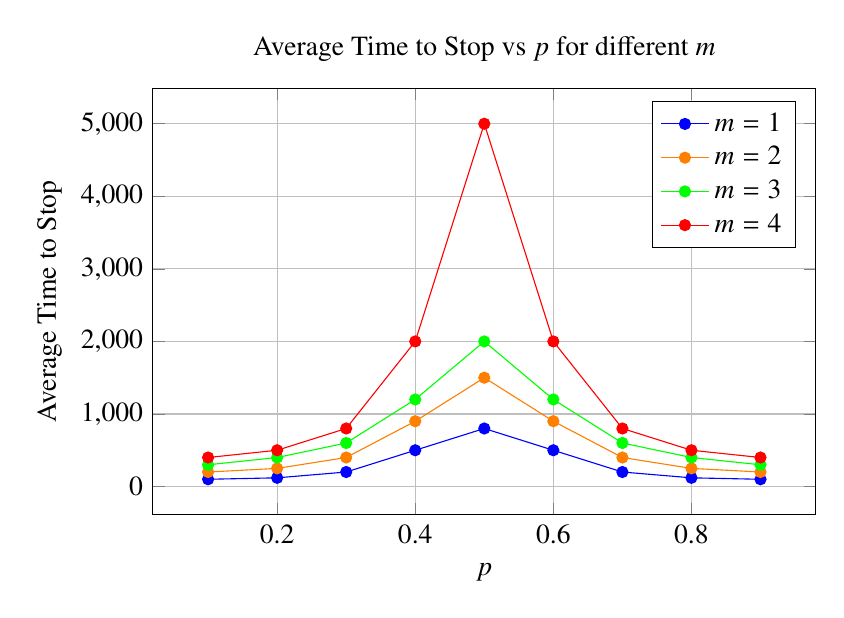
\begin{tikzpicture}
        \begin{axis}[
            title={Average Time to Stop vs $p$ for different $m$},
            xlabel={$p$},
            ylabel={Average Time to Stop},
            legend pos=north east,
            grid=major,
            width=10cm,
            height=7cm
        ]
        % Plot for m=1
        \addplot[
            color=blue,
            mark=*,
            ]
            coordinates {
            (0.1,100)(0.2,120)(0.3,200)(0.4,500)(0.5,800)(0.6,500)(0.7,200)(0.8,120)(0.9,100)
            };
        \addlegendentry{$m=1$}
        
        % Plot for m=2
        \addplot[
            color=orange,
            mark=*,
            ]
            coordinates {
            (0.1,200)(0.2,250)(0.3,400)(0.4,900)(0.5,1500)(0.6,900)(0.7,400)(0.8,250)(0.9,200)
            };
        \addlegendentry{$m=2$}
        
        % Plot for m=3
        \addplot[
            color=green,
            mark=*,
            ]
            coordinates {
            (0.1,300)(0.2,400)(0.3,600)(0.4,1200)(0.5,2000)(0.6,1200)(0.7,600)(0.8,400)(0.9,300)
            };
        \addlegendentry{$m=3$}
        
        % Plot for m=4
        \addplot[
            color=red,
            mark=*,
            ]
            coordinates {
            (0.1,400)(0.2,500)(0.3,800)(0.4,2000)(0.5,5000)(0.6,2000)(0.7,800)(0.8,500)(0.9,400)
            };
        \addlegendentry{$m=4$}
        
        \end{axis}
    \end{tikzpicture}
    \caption{Average Time to Stop vs $p$ for different values of $m$}
    \label{fig:avg_time_vs_p}
\end{figure}

\subsection{Adaptive}

The following figure shows the belief function amount after sending each query. 
\begin{figure}
    \centering
    \includegraphics[width=1\linewidth]{Adaptive_simulation.png}
    \caption{Adaptive scenario}
    \label{fig:enter-label}
\end{figure}

\begin{figure}
    \centering
    \includegraphics[width=1\linewidth]{Adaptive_simulation_6_2.png}
    \caption{Caption}
    \label{fig:enter-label}
\end{figure}

\begin{figure}
    \centering
    \includegraphics[width=1\linewidth]{Query_belief.png}
    \caption{Caption}
    \label{fig:enter-label}
\end{figure}


\vspace{2cm}
This approach aims to maintain the confidentiality of individual user data while providing sufficient information to accurately distinguish between two users.

\begin{Theorem}
\label{th:1}
    ...

\begin{proof}
Please refer to Appendix \ref{A:1}.
\end{proof}
\end{Theorem}

\begin{Theorem}
\label{th:2}
    ...
\begin{proof}
Please refer to Appendix \ref{A:2}.
\end{proof}
\end{Theorem}







%%%%%% 
%% Appendix:
%% If needed a single appendix is created by
%%
\newpage
\appendices

\section{Proof of Theorem \ref{th:1}}
\label{A:1}

Given a sequence of queries resulting in responses \( T_1, T_2, \ldots, T_n \), now assume the agent has only received the first answer which is $T_1$, so the probability distribution of having hypothesis $H_1$ or $H_0$ after receiving the first query is like the following:
\begin{align*}
    q_1 = P_{H_i|T_1} = \frac{\pi_iP_{T_1|H}}{P_{T_1}}, i \in {0,1}
\end{align*}

where $\pi_i$ is the initial belief for the hypothesis type. 

We can continue and write this distribution for $T_1, T_2$:

\begin{align*}
    & q_2 = P_{H_i|T_1,T_2} = \frac{P_{T_2|H_iT_1}P_{H_i|T_1}}{P_{T_2|T_1}}
    \\& = \frac{\pi_iP_{T_1|H_i}P_{T_2|H_iT_1}}{P_{T_1}P_{T_2|T_1}}
\end{align*}

By now we can calculate the likelihood ratio:

\begin{align*}
&\Lambda = \frac{\frac{\pi_0P_{T_1|H_0}P_{T_2|H_0T_1}}{P_{T_1}P_{T_2|T_1}}}{\frac{\pi_1P_{T_1|H_1}P_{T_2|H_1T_1}}{P_{T_1}P_{T_2|T_1}}}
= \frac{\pi_0P_{T_1|H_0}P_{T_2|H_0T_1}}{\pi_1P_{T_1|H_1}P_{T_2|H_1T_1}}
\end{align*}

\begin{align*}
    \frac{P_{T_1|H_0}P_{T_2|H_0T_1}}{P_{T_1|H_1}P_{T_2|H_1T_1}}>< \frac{\pi_1}{\pi_0}
\end{align*}

Now we can extend the result and find $\Lambda$ for the $n$th query:

\begin{align*}
    &\Lambda(T_n) = \Lambda (T_{n-1}) \times \frac{P(T_n|H_0, T_1, T_2, \dots T_{n-1})}{P(T_n|H_1, T_1, T_2, \dots T_{n-1})}
    \\& = \Lambda (T_{n-1}) \times \frac{P(T_n|H_0)}{P(T_n|H_1)}
\end{align*}

\subsection{Error Probability Non-adaptive}
The probability of error Type I is like the following:

\begin{align*}
    1-P_e = P(\frac{P_0(T^n)}{P_1(T^n)}<\eta| H_0)
\end{align*}

where $P_0,P_1$ are distribution on $T_n$ under hypothesis $H_0$ and $H_1$ respectively and $\eta \triangleq \frac{\pi_1}{\pi_0}$. 

If the current query is independent of the last queries we can write like the following:

\begin{align*}
    &1 - P_e = P (\frac{\prod_{i=1}^n P_0(T_i)}{\prod_{i=1}^n P_1(T_i)}>\eta | H_0)
    \\& = P (\frac{1}{n} \sum_{i=1}^n \log \frac{P_0(T_i)}{P_1(T_i)}> \frac{1}{n} \log \eta | H = 0)
\end{align*}

\begin{align*}
    \frac{1}{n} \sum_{i=1}^n \log \frac{P_1(T_i)}{P_0(T_i)} = \mathbb{E}_{H_0} \left[ \log \frac{P_1(T)}{P_0(T)} \right]
\end{align*}

\begin{align*}
    & 1 - P_e = P\left( \frac{1}{n} \sum_{i=1}^n \log \frac{P_0(T_i)}{P_1(T_i)}  - \mathbb{E}_{H_0} \left[ \log \frac{P_0(T)}{P_1(T)} \right] \right. \\
    & \left. > \frac{1}{n} \log \eta - \mathbb{E}_{H_0} \left[ \log \frac{P_0(T)}{P_1(T)} \right] \middle| H = 0 \right)
\end{align*}

Given that \(X_i = \log \frac{P_0(T_i)}{P_1(T_i)}\) and \(\mu = \mathbb{E}_{H_0} \left[ \log \frac{P_0(T)}{P_1(T)} \right]\), the error probability is:
\[
P\left( \frac{1}{n} \sum_{i=1}^n X_i - \mu > \frac{1}{n} \log \eta - \mu \middle| H = 0 \right)
\]

Given the sum \( S_n = \sum_{i=1}^n X_i \) and its expectation \( n\mu \), we want to bound the probability \( P\left( S_n - n\mu > \log \eta \right) \). Using the Chernoff bound, we have:

\[
P\left( S_n - n\mu > \log \eta \right) \leq \min_{t > 0} e^{-t(\log \eta + n\mu)} \cdot \left( \mathbb{E}[e^{tX_i}] \right)^n
\]


\subsection{Error Probability Adaptive}

Before sending a new query we update the $\pi_0, \pi_1$ based on our last answers, and from this point we implement the non-adaptive strategy.


 

\section{Proof of Theorem \ref{th:2}}

\section*{Theoretical Bound on the Error Exponent}

Given the error exponent 
\[
\Esf(\Qsf_K) = - \frac{1}{\mathbb{E} \left[ \sum_{k \in [K]} \mathsf{T}_{k}\right]}  \log \beta_K,
\]
we aim to find a theoretical bound by relating it to the information content of the queries and the distinguishability of the hypotheses.

Assuming the queries are optimally chosen to maximize the information gain about the hypotheses, the cumulative information gain across all queries can be approximated by the sum of Kullback-Leibler divergences between the probability distributions under the two hypotheses for each query-hit exchange. Formally, let $D(P_{X|Q_k} || P_{Y|Q_k})$ denote the KL divergence for the $k$-th query, then
\[
\mathcal{I}_{\text{cumulative}} = \sum_{k \in [K]} D(P_{X|Q_k} || P_{Y|Q_k}).
\]

Following the Chernoff-Stein Lemma, the error exponent for distinguishing between the two hypotheses is bounded by this cumulative information gain. Therefore,
\[
\Esf(\Qsf_K) \geq \frac{\mathcal{I}_{\text{cumulative}}}{\mathbb{E} \left[ \sum_{k \in [K]} \mathsf{T}_{k}\right]},
\]
where the expectation in the denominator reflects the average time required to accumulate this information.

This formulation highlights the trade-off between the speed of information acquisition and the accuracy of hypothesis discrimination.


\[
\Esf^* = \max_{\Qsf_K} \left\{ -\frac{1}{\mathbb{E}[\sum_{k=1}^K \mathsf{T}_k]} \log \beta_K \right\},
\]

subject to:

\[
\alpha_K \leq \epsilon,
\]

where \(\epsilon\) is the acceptable Type-I error rate, and the maximization is over all permissible sequences of queries \(\Qsf_K\) that adhere to the constraint.

\[
\Esf(\Qsf_K) \approx - \frac{C(H_0, H_1)}{\mathbb{E} \left[ \sum_{k \in [K]} \mathsf{T}_{k}\right]},
\]

where \(C(H_0, H_1)\) represents the Chernoff information between hypotheses \(H_0\) and \(H_1\), which serves as an approximation to the cumulative mutual information \(\mathcal{I}_{\text{cumulative}}\) gained from the sequence of \(K\) query-hit exchanges.

Given a querying strategy $\mathcal{Q}_K$ comprising $K$ queries, the objective is to maximize the error exponent $\Esf(\mathcal{Q}_K)$, defined by:

\[
\Esf(\mathcal{Q}_K) = - \frac{1}{\mathbb{E} \left[ \sum_{k=1}^{K} \mathsf{T}_k \right]} \log \beta_K,
\]

subject to:

\[
\alpha_K \leq \epsilon,
\]

where $\mathsf{T}_k$ denotes the hit-time for the $k$-th query, $\beta_K$ is the Type-II error probability, and $\alpha_K$ is the Type-I error probability with $\epsilon$ being the acceptable threshold.

The optimization problem can be further detailed as:

\[
\max_{\mathcal{Q}_K} \left\{ -\frac{1}{\mathbb{E} \left[ \sum_{k=1}^{K} \mathsf{T}_k \right]} \log \left( \sum_{k=1}^{K} I(Q_k; H | Z^{T_{k-1}}) \right) \right\},
\]

where $I(Q_k; H | Z^{T_{k-1}})$ represents the mutual information between the $k$-th query response and the hypothesis, given the prior observations.

This formulation aims to find the set of queries $\{Q_k\}_{k\in [K]}$ that optimizes the information gain about the hypotheses while minimizing the expected time to make a decision, all within the constraints of maintaining a Type-I error rate below $\epsilon$.
\begin{align*}
    \mathbb{E} \left[ \sum_{k=1}^{K} \mathsf{T}_k \right] = \sum_{k=1}^{K} \mathbb{E}[\mathsf{T}_k],
\end{align*}


    \[
\Esf(\Qsf_K) = - \frac{1}{\sum_{k=1}^{K} \mathbb{E}[\mathsf{T}_k]} \log \left( \sum_{k=1}^{K} \left( H(H | Z^{T_{k-1}}) - H(H | Q_k, Z^{T_{k-1}}) \right) \right),
\]

subject to:

\[
\alpha_K \leq \epsilon.
\]

\[
\Esf(\Qsf_K) \approx -\frac{1}{K\mu_T} \log \left( \exp\left(-\frac{\delta^2 K \bar{I}}{2\sigma_I^2}\right) \right),
\]

subject to:

\[
\Pr\left(S_K \geq (1 + \delta)K\mu_T\right) \leq \exp\left(-\frac{\delta^2 K \mu_T}{3\sigma_T^2}\right),
\]

\[
\Pr\left(G_K \leq (1 - \delta)K\bar{I}\right) \leq \exp\left(-\frac{\delta^2 K \bar{I}}{2\sigma_I^2}\right).
\]


\label{A:2}





\section{Various considerations}

\textbf{Example}
\begin{align*}
   & X \in \{0,1\}
    \\& Q \in \{00,01,10,11\}
    \\& P_X = Ber(p), P_Y = Ber(q)
    \\& H(T_X) = - \sum_t P_{T_X} (t) \log (P_{T_X}(t))
    \\& = -\sum_{X_1,X_2} \sum_t P_{T_x}(t| x_1,x_2)P(x_1,x_2) \log P_{T_x}(t)
    \\& = - \Bigg[ P_{T_x}(t=2| x_1,x_2 = 00)P(x_1,x_2 = 00) \log P_{T_x}(t=2)
    \\& + \sum_{X_1,X_2 = \{01, 11\}}\sum_{t>2} P_{T_x}(t| x_1,x_2)P(x_1,x_2) \log P_{T_x}(t)
    \\& + \sum_{X_1,X_2 = 10 }\sum_{t>2} P_{T_x}(t| x_1,x_2)P(x_1,x_2) \log P_{T_x}(t) \Bigg]
    \\& = -\Bigg[(1-p)^2\log(1-p)^2 
    \\& + \sum_{X_1,X_2 = \{01, 11\}} P(x_1x_2) \sum_{t>4} P_{T_X}(t-2)\log (P_{T_X}(t))
    \\& + P(x_3 =0)\sum_{t\geq3} P_{T_x}(t| 100) \log P_{T_x}(t) +P(x_3 =1)
    \\&\times \sum_{t\geq3} P_{T_x}(t| 101) \log P_{T_x}(t) \Bigg]
    \\& = -\Bigg[(1-p)^2\log(1-p)^2 +p(-D(T_X || T^{t+2}_X)-H_{T_X})
    \\&+(1-p)\log P_{T_X}(3) + p(-D(T_X|| T^{t+3}_X)-H(T_X))\Bigg]
\end{align*}

\begin{align}
    & (1-2p)H_{T_X} = -(1-p)^2\log(1-p)^2 +p(D(T_X || T^{t+2}_X))
    \\&-(1-p)\log P_{T_X}(3) + p(D(T_X|| T^{t+3}_X))
\end{align}

\begin{align}
    & (1-2q)H_{T_Y} = -(1-q)^2\log(1-q)^2 +q(D(T_Y || T^{t+2}_Y))
    \\&-(1-q)\log P_{T_Y}(3) + q(D(T_Y|| T^{t+3}_Y))\end{align}

\begin{align*}
    & D(P_X||P_Y) = \sum_{t\geq 2} P_{T_X=t} \log \frac{P_{T_X(t)}}{P_{T_Y}(t)} 
    \\& = \sum_{X_1,X_2}  \sum_{t\geq 2} P(T_X=t| X_1,X_2=x_1x_2) P(x_1,x_2) \log \frac{P_{T_X(t)}}{P_{T_Y}(t)} 
    \\& = P(T_X =2)\log \frac{P(T_X =2)}{P(T_Y =2)} 
    \\& + \sum_{t= 3} \sum_{X_1,X_2 \in \{01,11\}} P(x_1,x_2) P(T_X=t| X_1,X_2=x_1x_2) \log \frac{P_{T_X(t)}}{P_{T_Y}(t)} 
    \\& +\sum_{t= 3} \sum_{X_1,X_2 \in \{10\}} P(x_1,x_2) P(T_X=t| X_1,X_2=x_1x_2) \log \frac{P_{T_X(t)}}{P_{T_Y}(t)} 
    \\& = P(T_X =2)\log \frac{P(T_X =2)}{P(T_Y =2)} 
    \\& +  \sum_{X_1,X_2 \in \{01,11\}} P(x_1,x_2) \sum_{t\geq 3} P(T_X=t-2) \log \frac{P_{T_X(t)}}{P_{T_Y}(t)} 
    \\& +  \sum_{X_1,X_2 \in \{10\}} P(x_1,x_2)\sum_{t= 3} P(T_X=t-2) \log \frac{P_{T_X(t)}}{P_{T_Y}(t)} 
    \\&= P(T_X =2)\log \frac{P(T_X =2)}{P(T_Y =2)} 
    \\& +  p\sum_{t\geq 2} P(T_X=t) \log \frac{P_{T_X(t+2)}}{P_{T_Y}(t+2)} 
    \\& + P(x_3=0) \sum_{t= 3} P(t|100) \log \frac{P_{T_X(t)}}{P_{T_Y}(t)} + P(x_3=1) \sum_{t= 3} P(t|101) \log \frac{P_{T_X(t)}}{P_{T_Y}(t)} 
    \\& =  P(T_X =2)\log \frac{P(T_X =2)}{P(T_Y =2)} 
    \\& +  p( -D(T_X||T^{t+2}_X)+ D(T_X||T^{t+2}_Y))
    \\& +  P(T_X=3) \log \frac{P(T_X=3)}{P(T_Y=3)}+ p (-D(T_X|| T^{t+3}_X)+D(T_X||T^{t+3}_Y))
    \\& =  P(T_X =2)\log \frac{P(T_X =2)}{P(T_Y =2)}  + P(T_X=3) \log \frac{P(T_X=3)}{P(T_Y=3)}
    \\& +  p( -D(T_X||T^{t+2}_X)- D(T_X|| T^{t+3}_X))
    \\& +  p (D(T_X||T^{t+2}_Y)+D(T_X||T^{t+3}_Y))
\end{align*}

\begin{align*}
    & D(T_X||T^{t+2}_Y) = (1-p)^2 \log\frac{P_{T_X}(2)}{P_{T_Y}(4)} + p(D(T_X||T^2_X) - D(T_X||T^4_Y)
    \\& +(1-p) \log \frac{P_{T_X}(1)}{P_{T_Y}(5)} +p(D(T_X||T^3_X) - D(T_X||T^5_Y)
\end{align*}

\begin{align*}
    & D(T_X||T^{t+3}_Y) = (1-p)^2 \log\frac{P_{T_X}(2)}{P_{T_Y}(5} + p(D(T_X||T^3_X) - D(T_X||T^5_Y)
    \\& +(1-p) \log \frac{P_{T_X}(1)}{P_{T_Y}(6)} +p(D(T_X||T^4_X) - D(T_X||T^6_Y)
\end{align*}

SR 
\begin{enumerate}
    \item  scaling with the cardinality $\Zcal$
    \item  adding $\| \Zcal \| $ to the rate constraint scaling should allow one to compare across lengths
    \item  query/hit  or probe/echo or ping/response
\end{enumerate}

\bibliographystyle{unsrt}
\bibliography{References}
\end{document}



